\documentclass[conference]{IEEEtran}
\IEEEoverridecommandlockouts
% The preceding line is only needed to identify funding in the first footnote. If that is unneeded, please comment it out.
\usepackage{cite}
\usepackage{amsmath,amssymb,amsfonts}
\usepackage{algorithmic}
\usepackage{graphicx}
\usepackage{textcomp}
\usepackage{xcolor}
\usepackage{diagbox}
\usepackage{float}
\usepackage{multirow}
\def\BibTeX{{\rm B\kern-.05em{\sc i\kern-.025em b}\kern-.08em
    T\kern-.1667em\lower.7ex\hbox{E}\kern-.125emX}}
\begin{document}

\title{ Optimisation Naturelle : Une Exploration Approfondie de l'Algorithme Firefly\\
}

\author{\IEEEauthorblockN{ Anthony Wilhelm}
\IEEEauthorblockA{\textit{UHA 4.0} \\
\textit{Université de Haute Alsace}\\
Mulhouse , France \\
anthony.wilhelm@uha.fr}
}

\maketitle

\begin{abstract}
Afin d'accélérer l'exécution des divers algorithmes, les chercheurs en informatique ont trouvé inspiration dans les mécanismes naturels. Dans ce document, nous explorons une approche novatrice visant à optimiser le temps de calcul de fonctions qui, dans des conditions normales, exigeraient un temps d'exécution infini. Nous nous penchons sur la manière dont cette méthode, inspirée par les phénomènes naturels, peut considérablement améliorer l'efficacité des algorithmes, ouvrant ainsi de nouvelles perspectives dans le domaine de l'informatique et de l'optimisation.
\end{abstract}

\begin{IEEEkeywords}
Optimisatoion, Luciole, Algorithme, Benchmark
\end{IEEEkeywords}

\section{Introduction}

Dans le domaine informatique, l'optimisation est une discipline cruciale qui permet la réalisation efficace de calculs liés aux fonctions scientifiques. Notre attention se porte ici sur une approche particulière d'optimisation, à savoir l'algorithme Firefly, qui s'inspire du comportement social des lucioles. Ces insectes communiquent entre eux en utilisant des signaux lumineux pour attirer un partenaire, et cette inspiration naturelle offre une perspective unique dans le développement d'algorithmes.

Dans la suite de cet article, nous explorerons le fonctionnement détaillé de l'algorithme Firefly, examinant comment il émule les interactions lumineuses des lucioles pour optimiser des fonctions. Ensuite, nous partagerons les résultats obtenus lors de l'exécution de cet algorithme avec différentes fonctions de test telles que la sphère, la fonction de Restrigin, la fonction de Rosenbrock et la fonction d'Ackley. Cette analyse pratique nous permettra de mieux comprendre l'efficacité et la robustesse de l'algorithme Firefly dans la résolution de problèmes d'optimisation complexes liés aux fonctions scientifiques.

\section{Contextualisation de l'algorithme firefly}

\subsection{l'inspiration biologique des lucioles}


L'algorithme Firefly se distingue en tant qu'algorithme d'optimisation novateur intégrée par Xin-She Yang en 2008 qui tire son inspiration des phénomènes naturels, précisément du comportement social des lucioles. Dans la nature, ces insectes nocturnes utilisent des signaux lumineux pour communiquer entre eux, établir des liens sociaux et, notamment, attirer des partenaires. Cette forme de communication lumineuse a captivé les chercheurs en informatique, qui ont transposé ces principes dans le domaine de l'optimisation.

L'idée fondamentale derrière l'algorithme Firefly est de reproduire la manière dont les lucioles s'organisent dans l'espace en fonction de l'intensité de leurs lueurs. Chaque luciole, représentant une solution potentielle dans un espace d'optimisation, ajuste sa position en réponse à la luminosité des lucioles voisines. Cette interactivité est utilisée pour guider la convergence du groupe de lucioles vers une solution optimale.



\subsection{Algorithme "Firefly" en Action}

En intégrant ces phénomènes naturels dans le processus d'optimisation, l'algorithme Firefly propose une approche bio-inspirée, où la recherche de solutions se déroule de manière collective et adaptative. Cette conceptualisation unique offre un pont entre les stratégies d'optimisation informatique et les mécanismes observés dans la nature, ouvrant ainsi de nouvelles perspectives pour la résolution de problèmes complexes. En explorant les comportements sociaux des lucioles, l'algorithme Firefly devient un exemple concret de la manière dont les principes naturels peuvent être exploitées pour améliorer les performances des algorithmes d'optimisation.

\section{Manière dont les lucioles communiquent entre elles pour converger}
Les lucioles, agissant comme agents dans l'algorithme Firefly, communiquent entre elles par le biais d'interactions lumineuses pour converger vers une solution optimale. Ce mécanisme de communication simulé s'inspire du comportement naturel des lucioles, qui utilisent leurs signaux lumineux pour coordonner leurs actions dans un environnement nocturne. Chaque luciole émet une lumière dont l'intensité est proportionnelle à la qualité de la solution qu'elle représente. Ainsi, une luciole avec une luminosité plus élevée indique une solution de meilleure qualité.

Lors de chaque itération de l'algorithme, chaque luciole évalue l'attraction qu'elle ressent envers les autres lucioles en fonction de leur luminosité relative. Une luciole sera davantage attirée par celles émettant une lumière plus intense. Cette attraction est calculée en utilisant une fonction d'attraction, déterminée par le facteur d'absorption lumineuse et la distance entre les lucioles. 

Le processus de communication entre les lucioles se traduit par des ajustements dynamiques de leurs positions dans l'espace de recherche. Les lucioles se déplacent vers des positions qui maximisent leur attraction mutuelle, favorisant ainsi la convergence du groupe vers des configurations spatiales où la qualité globale des solutions est optimale.

La communication lumineuse entre les lucioles crée une dynamique collective, simulant la capacité du groupe à s'auto-organiser vers des solutions de qualité supérieure. Ce mécanisme favorise une exploration efficace de l'espace des solutions, les lucioles convergeant progressivement vers des régions où la concentration de solutions optimales est maximale. En résumé, la communication lumineuse des lucioles dans l'algorithme Firefly crée une synergie bio-inspirée qui guide le groupe vers une convergence collective, conduisant à la découverte de solutions optimales dans des problèmes d'optimisation complexes.

\begin{figure}[ht]
  \centering
  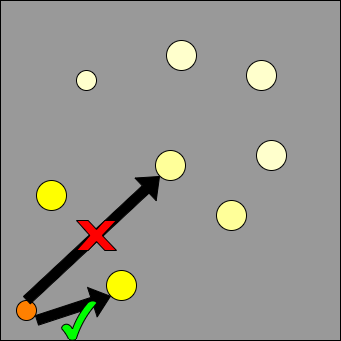
\includegraphics[width=8cm]{Attirance.png}
  \caption{Attirance des lucioles}
  \label{fig:enter-label}
\end{figure}

Cette illustration s'inspire d'une images des recherches menées par Andrey Dik (https://www.mql5.com/fr/articles/11873) sur l'algorithme des lucioles, également connu sous le nom de Firefly Algorithm (FA), telles que présentées dans son article intitulé "Algorithmes d'optimisation de la population : Algorithme des Lucioles". Dans ce travail, l'image met en lumière le concept fondamental d'attraction entre les lucioles, soulignant leur propension à être attirées les unes par les autres en fonction de leur proximité et de leur luminosité. L'analogie avec le comportement naturel des lucioles est utilisée pour illustrer la manière dont ces créatures virtuelles ajustent leur position dans l'espace de recherche, s'orientant vers des solutions potentiellement optimales à mesure qu'elles interagissent les unes avec les autres. Cette visualisation offre une représentation graphique captivante des principes bio-inspirés sous-jacents à l'algorithme des lucioles.

\section{Explication détaillée du fonctionnement de l'algorithme}

 Nous venons de voir que l'algorithme Firefly, inspiré du comportement social des lucioles. Explorons en détail le fonctionnement de cet algorithme, mettant en avant ses principaux concepts et mécanismes.

 \subsection{Initialisation}
 L'algorithme débute par la création d'une population de lucioles, chacune représentant une solution possible à un problème d'optimisation. Les positions initiales des lucioles sont générées de manière aléatoire dans l'espace de recherche, et leur qualité est évaluée en fonction de la fonction objectif.

 \subsection{Attraction et Mouvement}
 Le concept central de l'algorithme est l'attraction entre les lucioles. À chaque itération, chaque luciole évalue l'attraction qu'elle ressent envers les autres lucioles, en se basant sur la luminosité relative. Les lucioles sont attirées vers celles qui émettent une lumière plus intense. La mise à jour de la position d'une luciole est effectuée en fonction de cette attraction, ce qui favorise le mouvement vers des positions plus lumineuses dans l'espace de recherche.

 \subsection{Facteur d'absorption lumineuse}
 Le facteur d'absorption lumineuse $\beta$ joue un rôle crucial dans la modulation de l'attraction entre les lucioles. Il est initialisé à $\beta$0  et subit une décroissance au fil des itérations, ce qui représente une adaptation dynamique de la visibilité des lucioles. Ce mécanisme permet de réguler l'intensité des signaux lumineux et d'ajuster l'exploration de l'espace des solutions.


\subsection{Exploration et Convergence}
Les lucioles explorent l'espace de recherche de manière collaborative, se déplaçant vers des positions plus lumineuses. Ce processus simule la recherche collective de solutions optimales. Au fil des itérations, l'algorithme converge vers des configurations spatiales où les lucioles représentent des solutions de haute qualité.

\subsection {Mise à jour et évaluation}
Après chaque déplacement, la qualité des solutions est réévaluée, ajustant ainsi la luminosité des lucioles. La meilleure solution identifiée est conservée, et le processus itératif continue jusqu'à atteindre un critère d'arrêt prédéfini.

En résumé, l'algorithme Firefly combine l'idée d'une attraction sociale entre les lucioles, basée sur leur luminosité respective, avec des mécanismes d'adaptation dynamique (facteur d'absorption lumineuse) pour guider la recherche vers des solutions optimales. Ce processus bio-inspiré offre une approche puissante pour résoudre divers problèmes d'optimisation en exploitant des principes de la nature.

\begin{figure}[ht]
  \centering
  \includegraphics[width=8cm]{Diagramme_activité.png}
  \caption{Diagramme d'activité de l'algorithme des lucioles}\cite{b1}
  \label{fig:enter-label}
\end{figure}

\section{Modélisation Mathématique}


\subsection{Attraction entre deux lucioles}
L'attraction entre deux lucioles i et j est exprimée mathématiquement par une formule d'intensité lumineuse qui est la suivante:
\[ \beta{i,j} = \beta_0 e ^{-\gamma \text r^2{i,j}}(Z{i} -Z{j})  \] \cite{b2}

$\beta$ : C'est l'attraction entre les lucioles i et j . C'est la quantité par laquelle la position de la luciole i est ajustée enréponse à la luciole j. \\
$\beta_0$ : Il s'agit du facteur d'absorption lumineuse initial.Il représente la luminosité maximale initile d'une luciole. \\
$\gamma$ : C'est le coefficient de la décroissance de l'absorption lumineuse. Il détermine la vitesse à laquelle l'attraction décroit avec la distance. \\
r : C'est la distance euclidienne entre les positions des lucioles i et j dans l'espace de recherche, Cette distance est au carré dans l'exponentiel , ce qui signifie que les lucioles sont plus fortement attiré lorsque elles sont les plus proches.\\
Z{i} et Z{j} : Sont les distances entre les lucioles i et j

\subsection{Génération des populations initial}
Pour débuter l'algorithme il faut créer une population de base de taille désirée avec des placement aléatoire  on utilisera une attirance pour $\beta_0$ pour que toute les luciole est une luminosité de départ égale : 
\[\text x{t+1} = x{t}+\beta_0 e ^{-\gamma \text r^2} +  a\epsilon \]\cite{b2}

x{t+1} : C'est la composante de la position de la luciole t 
a$\epsilon$ : Est un terme de randomisation avec ces paramètre de randomisation. 

\subsection{Mouvement des lucioles les moins lumineuses vers les plus lumineuses}

Les lucioles sont attiré par les autres qui sont plus lumineuses ce qui est déterminé par : 

\[ \text x{i} = x{i}+\beta_0 e ^{-\gamma \text r^2{i,j}}(xj-xi)+ a\epsilon \] \cite{b2}

x{i} : position d'une luciole\\
x{j}  : position d'une seconde luciole \\

 En réorganisant le classement, la meilleure solution peut être identifiée parmi l'ensemble des lucioles, permettant ainsi de déterminer la solution optimale du problème d'optimisation considéré.\\
Le paramètre \(\gamma\) joue un rôle crucial dans la modélisation de la variation attractivité entre les lucioles. Sa valeur revêt une importance particulière dans la détermination de la vitesse à laquelle l'algorithme converge ainsi que dans le comportement global de l'algorithme. En effet, \(\gamma\) influence directement l'intensité de l'attraction entre les lucioles, impactant ainsi la dynamique du processus d'optimisation. La sélection judicieuse de la valeur de \(\gamma\) est donc essentielle pour ajuster les performances de l'algorithme.\cite{b3}\\
Ces formulations mathématiques encapsulent les règles fondamentales de l'algorithme des lucioles, permettant une représentation précise de la manière dont les lucioles interagissent et comment leurs positions évoluent au fil du temps. Ces équations définissent les mécanismes essentiels qui guident la recherche vers des solutions optimales dans l'espace de recherche défini par le problème d'optimisation.



\section{Méthodologie Expériementale}
\subsection{Installtions}


Pour manipuler cet algorithme, l'utilisation de la bibliothèque Python "mealpy" est demandée. Cette bibliothèque propose une implémentation intégrée et encapsuler de l'algorithme FireFly (FFA dans la librairie).

Des évaluations de performance on été faite à partir de deux langage :
\begin{itemize}
    \item Python : C'est un langage qui dispose d'un ecosytème de de bibliothèque plutot puissant telles que Numpy, SciPy et Matplotlib (affichage de graphe) simplifiant les opérations numérique les calculs scientifique et les visualisations des résultats. 
    \item C++ :  C++ est réputé pour ses performances élevées. Si  l'algorithme des lucioles doit être exécuté de manière intensive ou sur des ensembles de données volumineux, la performance accrue de C++ peut être un avantage.C'est aussi un langage très utilisée dans le domaine de la recherche en informatique. 
\end{itemize}
La bibliothèque "mealpy" étant initialement conçue en langage Python, sa réutilisation pour les évaluations s'est avérée impossible. Avant de pouvoir procéder aux évaluations de performance, une conversion de la bibliothèque "mealpy" vers le langage C++ a été nécessaire (j'aurais malheureusement un biais dans mes expérimentation car je n'ai pas réussi à traduire l'algorithme en C++ en respectant la structure de la bibliothèque dans le temp imparti). Les mesures de performances ont étés effectué sur des fonctions souvent utilisée pour ça dans le milieu de l'optimisation. 

\subsection{Les fonctions tester}
\begin{itemize}
    \item La fonctions sphère :  La fonction sphère vise à évaluer la capacité d'un algorithme d'optimisation à trouver le minimum global. La fonction sphère a une forme géométrique qui ressemble à une sphère dans un espace multidimensionnel. Chaque composante contribue à la distance au carré par rapport à l'origine, et la somme totale de ces distances donne la valeur de la fonction. Représentation mathématique : \[ f(x) =\sum_{i=1}^{D} x_i^2\]

    \item La fonction Ackley : La fonction d'Ackley est connue pour sa complexité et son comportement multimodal, ce qui signifie qu'elle possède plusieurs optima locaux. Elle est souvent utilisée pour tester la capacité d'un algorithme d'optimisation à échapper aux minima locaux et à converger vers le minimum global. Représentation mathématique :{\tiny \[f(x) = -a \cdot \exp\left(-b \sqrt{\frac{1}{D} \sum_{i=1}^{D} x_i^2}\right) - \exp\left(\frac{1}{D} \sum_{i=1}^{D} \cos(c \cdot x_i)\right) + a + \exp(1)\]}

    \item La fonction Rastrigin : La fonction de Rastrigin est caractérisée par sa nature multimodale, ce qui signifie qu'elle présente plusieurs optima locaux, créant des difficultés pour les algorithmes d'optimisation qui peuvent être piégés dans des minimums locaux. Représentation mathématique  :\[f(x) = A \cdot D + \sum_{i=1}^{D} \left( x_i^2 - A \cdot \cos(2\pi x_i) \right)\]
    
    \item La fonction Rosenbrock : La fonction de Rosenbrock a une forme en "vallée" allongée, ce qui la rend intéressante pour tester les algorithmes d'optimisation. Il s'agit de minimiser la fonction dans une étroite vallée avec une solution optimale à l'intérieur.RosenBrock est utilisée pour évaluer la capacité des algorithmes d'optimisation à naviguer à travers des vallées allongées et converger vers le minimum global. Elle teste la robustesse des algorithmes face à des problèmes de convergence lente et à des régions difficiles de l'espace de recherche. Représentation mathématique : \[f(x) = \sum_{i=1}^{D-1} \left( 100 \cdot (x_{i+1} - x_i^2)^2 + (1 - x_i)^2 \right)\]

\end{itemize}
\subsection{Protocole expérimentale}
Pour chacun des langage et afin d'obtenir des résultats significatifs tout en évitant des temps d'exécutions excessivement longs, les fonctions ont été testées avec 5000 époques pour 10 itérations. Trois ensembles de tests ont été réalisés, chacun avec une population de 30, 50 et 70 individus, et pour chaque population, les tests ont été menés avec 10, 30 et 50 dimensions toutes les fonctions ont été testée avec des bornes de [-10,10] .\\
Les résultats ont été enregistrés dans un fichier Excel pour faciliter le calcul des moyennes, des écarts-types, et l'identification de tendances significatives.


\section{Les résultats}

Les différents graphiques ci-dessous montrent les résultats obtenus pour les neuf cas possibles qui ont été étudiés. L'ordre des dimensions est croissant, donc les trois premiers résultats concernent une taille de population de 30, les trois suivants pour 50, et les trois derniers pour une population de 70. Les dimensions sont toujours répertoriées dans le même ordre : 10, 30, 50.

\begin{figure}[H]
  \centering
  \includegraphics[width=8cm]{Sphere.png}
  \caption{\textbf{Moyenne des 1O meilleurs résultat obtenue pour chacun des cas étudier avec la fonction Sphère} }
  \label{fig:enter-label}
\end{figure}

\begin{figure}[H]
  \centering
  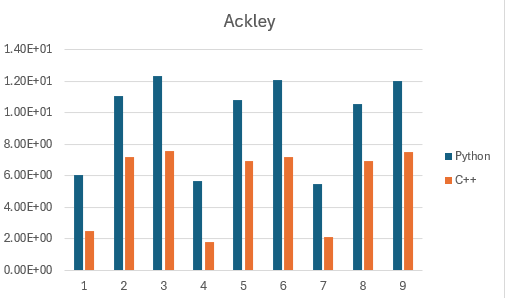
\includegraphics[width=8cm]{Ackley.png}
  \caption{\textbf{Moyenne des 1O meilleurs résultat obtenue pour chacun des cas étudier avec la fonction Ackley}}
  \label{fig:enter-label}
\end{figure}

\begin{figure}[H]
  \centering
  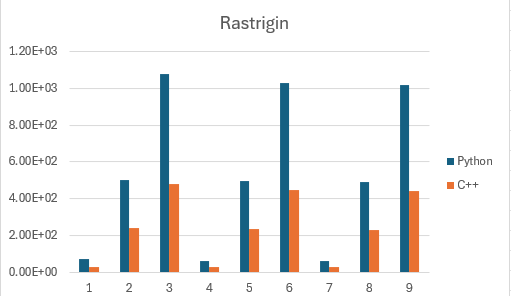
\includegraphics[width=8cm]{rastrigin.png}
  \caption{\textbf {Moyenne des 1O meilleurs résultat obtenue pour chacun des cas étudier avec la fonction Rastrigin}}
  \label{fig:enter-label}
\end{figure}


\begin{figure}[H]
  \centering
  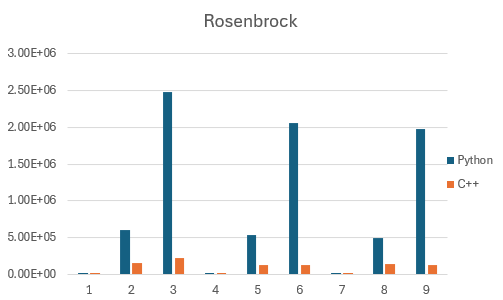
\includegraphics[width=8cm]{rosenbrock.png}
  \caption{\textbf {Moyenne des 1O meilleurs résultat obtenue pour chacun des cas étudier avec la fonction Rosenbrock}}
  \label{fig:enter-label}
\end{figure}

\subsection{Observation des résultats}

On observe que les différentes fonctions renvoient des valeurs qui varient considérablement en termes d'ordres de grandeur. Les valeurs les plus élevées sont atteintes par la fonction Rosenbrock, tandis que les valeurs les plus basses sont données par la fonction Ackley. Il est notable que, pour les fonctions Rosenbrock, Rastrigin et Ackley, une différence significative de performance de l'algorithme des lucioles est observée. On constate une disparité importante, jusqu'à un ordre de grandeur de $10^3$, entre les valeurs renvoyées par l'algorithme dans les langages Python et C++.Entre les fonctions on observe des différence d'ordre de grandeur $10^6$. Pour la fonction sphère, les résultats sont généralement similaires entre les deux langage, à l'exception d'un cas particulier étudié avec une population de 70 individus et 50 dimensions, où l'on observe une nette différence avec les résultats en Python qui s'envolent.

\subsection{Critique des résultats}

La différence notable entre les deux langages, outre leur rapidité d'exécution, peut résider dans la graine utilisée pour générer les nombres aléatoires, qui n'a pas été fixée. De plus, il est important de noter que les deux programmes n'ont pas été lancés simultanément.


Il est observé que l'algorithme peut converger vers une valeur proche de zéro avec des fonctions objectifs, mais présente souvent des pics importants. Cette tendance pourrait être attribuée au nombre limité d'époques utilisé lors des expérimentations, fixé à seulement 5000. Un tel nombre d'époques peut être insuffisant pour permettre à l'algorithme d'explorer de manière approfondie l'espace de recherche et d'atteindre une convergence plus stable.

Pour obtenir une évaluation plus robuste de la convergence de l'algorithme, il pourrais être intéressant d'augmenter le nombre d'époques à un niveau plus élevé.. Une expérimentation prolongée pourrait permettre une exploration plus exhaustive de l'espace de recherche, potentiellement conduisant à une meilleure identification de la solution optimale.

Cette extension du nombre d'époques pourrait aider à atténuer les pics observés, offrant ainsi une vue plus claire de la performance de l'algorithme sur la fonction objectif. Il est conseillé de réaliser des essais avec différents niveaux d'époques pour évaluer la sensibilité de l'algorithme à ce paramètre et pour déterminer le point optimal entre le temps de calcul disponible et la qualité de la solution recherchée.\\

\textbf{Table 1  : Benchmark :Moyennes sur 10 itérations des meilleurs des des résultats de 30,50,70 de population et 10,30,50 de dimension avec le langage C++ ainsi que les 4 fonctions tester et }

\begin{figure}[H]
  \centering
  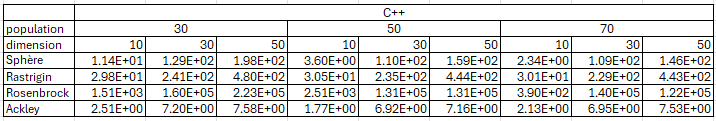
\includegraphics[width=10cm , height =3cm]{tabC.png}
  
\end{figure}
\newpage

\textbf{Table 2  : Benchmark :  Moyennes sur 10 itérations des meilleurs des des résultats de 30,50,70 de population et 10,30,50 de dimension avec le langage Python ainsi que les 4 fonctions tester et }
\begin{figure}[H]
  \centering
  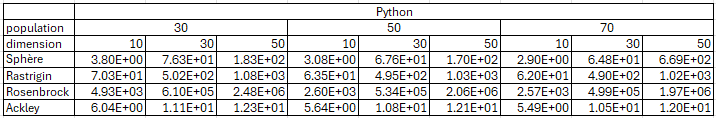
\includegraphics[width=9cm , height =3cm]{tabpy.png}
  
\end{figure}

\textbf{Table 2  : Benchmark :  Moyennes sur 10 itérations des Écart-types de 30,50,70 de population et 10,30,50 de dimension avec le langage Python ainsi que les 4 fonctions tester et }
\begin{figure}[H]
  \centering
  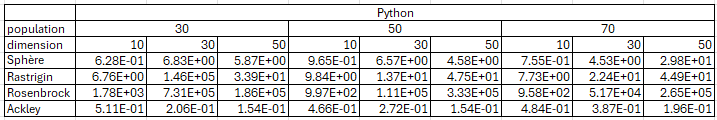
\includegraphics[width=9cm , height =3cm]{tabPyE.png}
  
\end{figure}


\textbf{Table 2  : Benchmark :  Moyennes sur 10 itérations des Écart-types de 30,50,70 de population et 10,30,50 de dimension avec le langage C++ ainsi que les 4 fonctions tester et }
\begin{figure}[H]
  \centering
  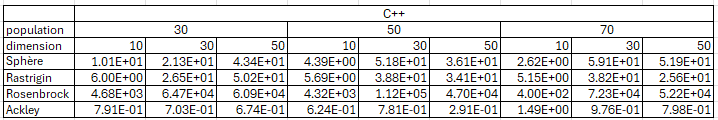
\includegraphics[width=9cm , height =3cm]{TabCEC.png}
  
\end{figure}









\subsection{Conclusion}
En conclusion les algorithmes bio-inspirée permettent de grande avancée dans le monde de l'optimisation en informatique en s'inspirant de phénomène naturel comme dans notre exemple les lucioles qui attirent des partenaires pour s’accoupler ou des victimes potentielles. Chaque phénomène peut être utile en fonction du cas on s'en ai bien rendu compte avec les expérimentations effectuée que en fonction de la fonction objectifs les résultats étais plus ou moins bon . Ce qui montre bien la limite de l'utilisation de ces algorithme qui seront les meilleurs dans des cas d'utilisations précis  l'algorithme des lucioles a par exemples été utilisé pour résoudre un problème dans le domaine du soin a domicile \cite{b4}. 











\begin{thebibliography}{00}
    \bibitem{b1} Krishna Durbhaka, Gopi \& Selvaraj, Barani \& Nayyar, Anand. (2019). Firefly Swarm: Metaheuristic Swarm Intelligence Technique for Mathematical Optimization: Proceedings of ICDMAI 2018, Volume 2. 10.1007/978-981-13-1274-8\_34.\\
    \bibitem{b2} Balande, U. Shrimankar, D. SRIFA: Stochastic Ranking with Improved-Firefly-Algorithm for Constrained Optimization Engineering Design Problems. Mathematics 2019, 7, 250.\\
    \bibitem{b3} Beghoura Mohamed Amine, mémoire : Segmentation multi sources des images Satellitaire par l'algorithme Firefly, UNIVERSITE DES SCIENCES ET DE LA TECHNOLOGIE d’ORAN, 2012.\\
    \bibitem{b4} Latifa Dekhici, Rabeh Redjem, Khaled Belkadi, Abderrahman El Mhamedi. Algorithme de Lucioles pour le Soin à Domicile. Internationnal conference on complex systems and logistic; ICOSYL 2018, Apr 2018, Paris, France. ffhal-02473691f\\
\end{thebibliography}






\end{document}
